\documentclass[a4paper, 11pt]{article}

\usepackage[utf8]{inputenc}
\usepackage[english]{babel}

\usepackage{hyperref}

\usepackage{graphicx}
\usepackage{float}

\usepackage{fullpage}

\begin{document}
	\begin{centering}
		\large\textbf{Progress Report: 24/01/2017}\\
		~\\
		Oussama ENNAFII:
		\normalsize MATIS | TITANE \\
		Directors: Cl\'ement Mallet \& Florent Lafarge \\
	\end{centering}


	\section*{Data:}
	
	\begin{itemize}
		\item Available data:
			\begin{itemize}
				\item[-] Bati3D data mostly in 3DS format on: Aix, Annecy, Elancourt, Lambesc, Lyon, Montpellier, Nantes, Paris and Toulouse;
				\item[-] DSM on regions: Toulouse, Elancourt and Nantes; Lambesc needs special application;
				\item[-] BD Ortho (HR) on: Toulouse, Aix, Elancourt, Lambesc and Nantes;
				\item[-] BD topo on: Toulouse.
			\end{itemize}
		\item Misc:
			\begin{itemize}
				\item[-] I need to adapt my script for other XML formats and for tar file handling,
				\item[-] Corrected Bati3D: February, 9th 2017, I am having an appointement with Yannick Couturier (DPR).
			\end{itemize}
	\end{itemize}
	
	\section*{Implementation:}
	I have implemented most of the library to handle 3D data:
	\begin{itemize}
		\item Implemented:
			\begin{itemize}
				\item[-] Reader: 3DS and OFF,
				\item[-] Geomview viewer,
				\item[-] Automated testing;
				\item[-] Algorithms on bricks: area, contour length, affine transformations.
			\end{itemize}
		\item To add:
			\begin{itemize}
				\item[-] Prune Bricks into Buildings and Terrains,
				\item[-] Visualize projections;
			\end{itemize}
		\item To complete:
			\begin{itemize}
				\item[-] Algorithms on bricks: projections (XY and Camera).
				\item[-] Handle KML, Collada and cityGML : I am curently in the process of dicussing this with Antoine Lavenant (D2SI),
				\item[-] Improve logging.
			\end{itemize}
	\end{itemize}
	
	\begin{figure}[H]
		\caption{\label{diag::class} Class diagram.}
		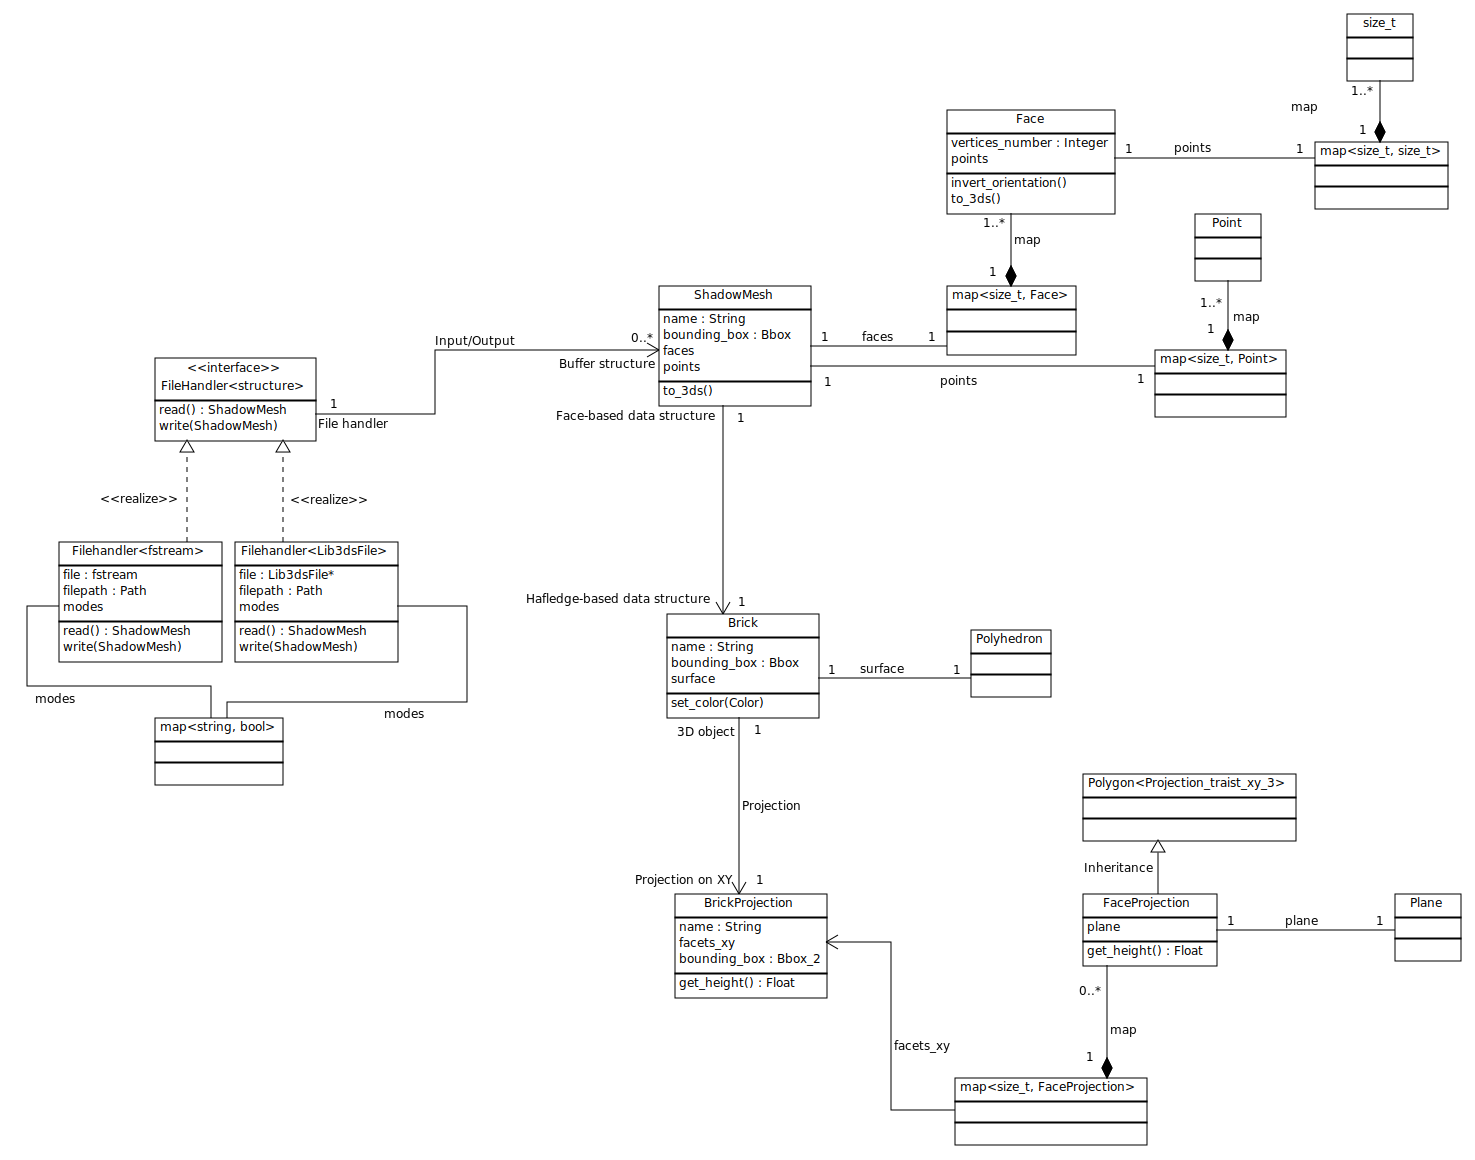
\includegraphics[scale=.3]{images/vectorial/class_diagram.png}
	\end{figure}
	
	\section*{Ideas:}
	There is nothing to report from the last time.
	
	\section*{Results:}
	There is no results to report for now.
	
	\section*{Attachments:}
	
	You can checkout the Code in \href{https://github.com/Ethiy/3DSceneModel}{Github}.
	
\end{document}
